\documentclass[11pt,a4paper]{article}

% ── Packages ────────────────────────────────────────────────────────────────
\usepackage[utf8]{inputenc}
\usepackage[T1]{fontenc}
\usepackage{lmodern}
\usepackage{geometry}
\usepackage{graphicx}
\usepackage{amsmath}
\usepackage{amssymb}
\usepackage{booktabs}
\usepackage{longtable}
\usepackage{array}
\usepackage{multirow}
\usepackage{xcolor}
\usepackage{colortbl}
\usepackage{hyperref}
\usepackage{listings}
\usepackage{fancyhdr}
\usepackage{titlesec}
\usepackage{enumitem}
\usepackage{float}
\usepackage{caption}
\usepackage{subcaption}
\usepackage{tikz}
\usetikzlibrary{shapes.geometric, arrows.meta, positioning, fit, backgrounds}
\usepackage{url}
\usepackage{setspace}
\usepackage{parskip}
\usepackage{microtype}

% Figures resolution order:
%   1. figures/                — Overleaf upload layout
%   2. ../output/figures/      — local repo layout
\graphicspath{{figures/}{../output/figures/}}

% ── Page geometry ────────────────────────────────────────────────────────────
\geometry{
  a4paper,
  top=2.5cm,
  bottom=2.5cm,
  left=3cm,
  right=2.5cm
}

% ── Colors ───────────────────────────────────────────────────────────────────
\definecolor{primaryblue}{RGB}{30, 56, 100}
\definecolor{accentblue}{RGB}{46, 91, 138}
\definecolor{lightgray}{RGB}{245, 245, 245}
\definecolor{medgray}{RGB}{200, 200, 200}
\definecolor{codegreen}{RGB}{40, 120, 40}
\definecolor{codegray}{RGB}{128, 128, 128}
\definecolor{codepurple}{RGB}{140, 0, 210}
\definecolor{codeblue}{RGB}{0, 0, 180}
\definecolor{rowblue}{RGB}{255, 255, 255}

% ── Hyperref setup ───────────────────────────────────────────────────────────
\hypersetup{
  colorlinks=false,
  linkcolor=black,
  citecolor=black,
  urlcolor=black,
  pdfborder={0 0 0},
  pdftitle={The AI Divide: Discovering Developer Archetypes},
  pdfauthor={CENG790 Big Data Analytics}
}

% ── Section title formatting ─────────────────────────────────────────────────
\titleformat{\section}
  {\Large\bfseries\color{black}}
  {\thesection.}{0.8em}{}[\titlerule]

\titleformat{\subsection}
  {\large\bfseries\color{black}}
  {\thesubsection.}{0.6em}{}

\titleformat{\subsubsection}
  {\normalsize\bfseries\color{black}}
  {\thesubsubsection.}{0.5em}{}

% ── Header / footer ──────────────────────────────────────────────────────────
\pagestyle{fancy}
\fancyhf{}
\fancyhead[L]{\small\textit{CENG790 --- Big Data Analytics}}
\fancyhead[R]{\small\textit{The AI Divide}}
\fancyfoot[C]{\thepage}
\renewcommand{\headrulewidth}{0.4pt}
\renewcommand{\footrulewidth}{0pt}

% ── Code listing style ───────────────────────────────────────────────────────
\lstdefinestyle{scala}{
  language=Scala,
  backgroundcolor=\color{lightgray},
  commentstyle=\color{codegreen}\itshape,
  keywordstyle=\color{codeblue}\bfseries,
  numberstyle=\tiny\color{codegray},
  stringstyle=\color{codepurple},
  basicstyle=\ttfamily\footnotesize,
  breakatwhitespace=false,
  breaklines=true,
  captionpos=b,
  keepspaces=true,
  numbers=left,
  numbersep=5pt,
  showspaces=false,
  showstringspaces=false,
  showtabs=false,
  tabsize=2,
  frame=single,
  rulecolor=\color{medgray},
  xleftmargin=15pt
}
\lstset{style=scala}

% ── Spacing ──────────────────────────────────────────────────────────────────
\onehalfspacing

% ════════════════════════════════════════════════════════════════════════════
\begin{document}
% ════════════════════════════════════════════════════════════════════════════

% ── Title page ───────────────────────────────────────────────────────────────
\begin{titlepage}
  \centering
  \vspace*{1cm}

  {\large\bfseries CENG790 --- BIG DATA ANALYTICS}\\[0.4cm]
  {\large PROJECT REPORT}\\[1.5cm]

  \rule{\linewidth}{2pt}\\[0.4cm]
  {\Huge\bfseries
    The AI Divide:\\[0.3cm]
    \large\bfseries Discovering Developer Archetypes from\\
    AI-Tool Adoption and their Impact on Compensation
  }\\[0.4cm]
  \rule{\linewidth}{2pt}\\[2cm]

  {\large\itshape A Big Data pipeline study using Apache Spark \& Scala\\
  on the 2024 Stack Overflow Developer Survey}\\[2cm]

  % ── Authors (REPLACE with real names) ─────────────────────────────────────
  \begin{tabular}{c@{\hspace{1.5cm}}c}
    {\large\bfseries First Author Name} & {\large\bfseries Second Author Name} \\[0.15cm]
    {\small Student ID 1}               & {\small Student ID 2} \\[0.10cm]
    {\small\texttt{author1@example.com}} & {\small\texttt{author2@example.com}} \\
  \end{tabular}

  \vspace{2cm}

  \begin{tabular}{rl}
    \textbf{Course}   & CENG790 --- Big Data Analytics \\[0.2cm]
    \textbf{Dataset}  & Stack Overflow Developer Survey 2024 ($N=65{,}437$) \\[0.2cm]
    \textbf{Pipeline} & Apache Spark 3.2.4 / Scala 2.12 / Spark MLlib \\[0.2cm]
    \textbf{Date}     & May 2026 \\
  \end{tabular}

  \vfill
  {\small This report describes a distributed Big Data pipeline that discovers
  three latent developer archetypes from real survey data and quantifies
  their impact on compensation, controlling for experience, geography and role.
  All artefacts are reproducible from a single \texttt{sbt run}.}
\end{titlepage}

% ── Abstract page ────────────────────────────────────────────────────────────
\begin{abstract}
\noindent
We use \textbf{distributed unsupervised learning on Apache Spark} to discover
latent developer archetypes from the 2024 Stack Overflow Developer Survey
($N=65{,}437$ raw $\to$ $13{,}552$ cleaned). Clustering on nine ordinal
features that describe AI adoption, sentiment, experience, and company
context, K-Means with $k=3$ recovers three distinct archetypes ---
\textit{Traditional Engineer}, \textit{AI Experimenter}, \textit{AI Power
User} --- with a silhouette score of $0.40$. We then test the popular claim
that \emph{AI Power Users earn less} against three confounds: experience,
geography, and developer role. The aggregate salary gap (Traditional
Engineers earn $\approx\$94$k versus Power Users $\$79$k) is shown to be a
\textbf{Simpson's paradox}: among juniors the gap is real and monotonic
($-\$12$k from None to Heavy AI use), but among seniors it
\textbf{reverses} ($+\$4$k--$9$k). A Spark MLlib linear regression with
experience and org-size controls cleanly decomposes the effect: trying more
AI \emph{products} raises salary ($+\$853$ per product, $p=0.05$), while
delegating more \emph{tasks} to AI lowers it ($-\$921$ per task, $p=0.001$).
The headline finding is therefore not ``AI hurts pay'' but ``task-offloading
does, tool-curiosity does not --- and the population-level gap is mostly a
confound of where AI tools are concentrated.''
\end{abstract}

\tableofcontents
\newpage

% ════════════════════════════════════════════════════════════════════════════
\section{Introduction}
% ════════════════════════════════════════════════════════════════════════════

The 2023--2025 wave of generative-AI tooling has put coding assistants in
front of every working developer. Public discourse has split into two
narratives: a \textbf{hype} narrative, in which vendors and influencers
claim AI tools deliver large productivity and salary upsides, and a
\textbf{skepticism} narrative, in which engineers warn of skill erosion,
lower-quality output, and that adoption may concentrate in less-technical
roles. This project asks whether that split is mathematically discoverable
in real survey data, and whether membership in any AI-adoption archetype
materially changes a developer's compensation, satisfaction, or work
arrangement.

\subsection{Research question}

\begin{quote}\itshape
  Can we use distributed unsupervised machine learning to discover latent
  developer archetypes --- ranging from ``AI Power Users'' to ``Traditional
  Engineers'' --- within the global software development community? Once
  these distinct profiles are identified, how do they impact an individual
  developer's annual compensation (\texttt{ConvertedCompYearly}) and job
  satisfaction (\texttt{JobSat}), after controlling for the obvious
  confounds of experience, country and role?
\end{quote}

\subsection{Contributions}

\begin{enumerate}[leftmargin=2em]
  \item A reproducible \textbf{end-to-end Spark/Scala pipeline} that
        ingests the raw 152\,MB CSV, builds a feature vector tailored to
        AI adoption, performs K-Means clustering, and emits a
        multi-section impact report (CSV $+$ Parquet) suitable for
        downstream visualisation.
  \item Empirical evidence that \textbf{three latent archetypes} exist with
        a silhouette of $0.40$ on the cleaned 9-dimensional feature space.
  \item A \textbf{deep-dive impact analysis} that controls for experience,
        geography and role, exposing a \textbf{Simpson's paradox} in the
        headline ``AI Power Users earn less'' claim and offering a more
        defensible replacement: heavy AI \emph{task-offloading} is
        associated with lower pay even after controlling for experience
        and org size, but the number of AI \emph{tools tried} has the
        opposite (small positive) effect.
\end{enumerate}

% ════════════════════════════════════════════════════════════════════════════
\section{Dataset}
% ════════════════════════════════════════════════════════════════════════════

\subsection{Source and overview}

We use the \textbf{Stack Overflow Annual Developer Survey 2024}, publicly
available at \url{https://survey.stackoverflow.co}. This is one of the most
comprehensive surveys of the global developer community.

\begin{table}[H]
\centering
\caption{Dataset overview}
\begin{tabular}{ll}
\toprule
\textbf{Property}       & \textbf{Value} \\
\midrule
Survey year             & 2024 \\
Total respondents       & 65{,}437 \\
Countries represented   & 185 \\
Total columns           & 114 \\
File format             & CSV (\texttt{survey\_results\_public.csv}) \\
File size               & $\approx 152$\,MB \\
License                 & Open Database License (ODbL) \\
\bottomrule
\end{tabular}
\end{table}

\subsection{Schema challenges in the 2024 survey}

The 2024 dataset materially differs from earlier versions; the cleaning
module had to be schema-aware:

\begin{table}[H]
\centering
\caption{2024-specific schema idiosyncrasies handled by the cleaning stage}
\rowcolors{2}{rowblue}{white}
\begin{tabular}{p{4.6cm}p{8cm}}
\toprule
\textbf{Field} & \textbf{2024 idiosyncrasy} \\
\midrule
\texttt{AIToolCurrently Using} & Column name contains a space, and lists
\textit{activities} (writing code, debugging, \ldots) --- \textbf{not} AI
products. \\
\texttt{AISearchDevHaveWorkedWith} & The actual list of AI products
(ChatGPT, GitHub Copilot, \ldots). \\
\texttt{JobSat} & Numeric 0--10 score (older versions used 5-level Likert
text labels). \\
\texttt{AIBen} & Multi-value semicolon list (e.g.~\textit{``Increase
productivity;Greater efficiency''}), not a single Likert label. \\
\texttt{AISelect} & New phrasing: \textit{Yes} / \textit{No, but I plan to
soon} / \textit{No, and I don't plan to}. \\
\texttt{OrgSize} & Includes \textit{``I don't know''} --- dropped to null. \\
\bottomrule
\end{tabular}
\end{table}

\subsection{Cleaning and filtering}

Sequential filters in \texttt{Cleaning.scala}:

\begin{enumerate}[leftmargin=2em]
  \item Keep only respondents whose \texttt{Employment} field contains
        \textit{``Employed, full-time''}.
  \item Drop rows with null \texttt{ConvertedCompYearly}, \texttt{JobSat},
        or \texttt{AISelect}.
  \item Cast salary to \texttt{Double}, drop salaries below \$5{,}000 or
        above \$1{,}000{,}000 as implausible.
  \item Normalise \texttt{YearsCodePro} (handle the
        \textit{``More than 50 years''} / \textit{``Less than 1 year''}
        string sentinels).
  \item Encode \texttt{OrgSize} (1--9), \texttt{JobSat} (0--10),
        \texttt{AISelect} (0--2), \texttt{AIAcc} (0--4), \texttt{AIThreat}
        (0--2), \texttt{AISent} (0--4) as ordinal integers.
  \item Convert the multi-value \texttt{AIBen} to \texttt{ai\_ben\_count}
        (number of distinct benefits selected).
\end{enumerate}

After cleaning, \textbf{13{,}552 rows} remain.

% ════════════════════════════════════════════════════════════════════════════
\section{Methodology}
% ════════════════════════════════════════════════════════════════════════════

\subsection{Pipeline architecture}

The full analysis is implemented as a five-stage distributed Big Data
pipeline using Apache Spark 3.2.4 and Scala 2.12.
Figure~\ref{fig:pipeline} illustrates the architecture.

\begin{figure}[H]
\centering
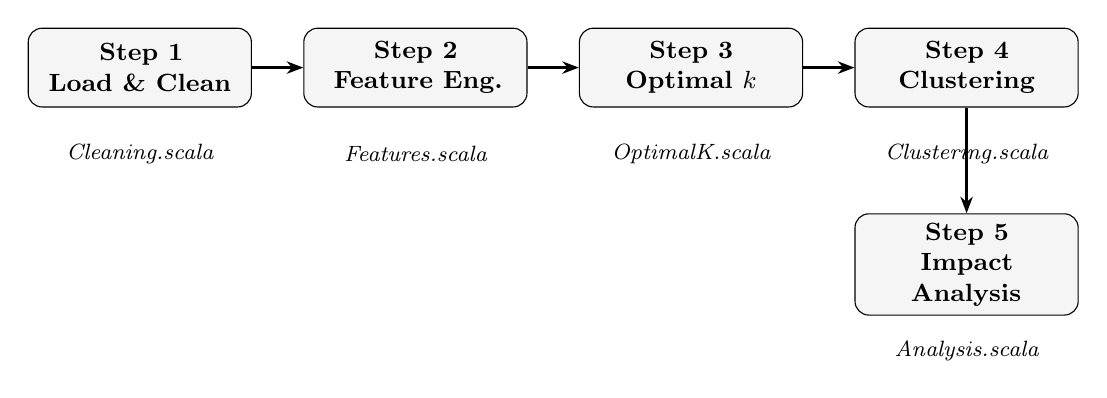
\begin{tikzpicture}[
  box/.style={rectangle, rounded corners=5pt, draw=black,
              fill=lightgray, minimum width=2.8cm, minimum height=1cm,
              text centered, font=\small\bfseries, text width=2.6cm},
  arrow/.style={-{Stealth[length=6pt]}, thick, color=black},
  label/.style={font=\footnotesize\itshape, color=black}
]
  \node[box] (load)    at (0,0)   {Step 1\\Load \& Clean};
  \node[box] (feat)    at (3.5,0) {Step 2\\Feature Eng.};
  \node[box] (optk)    at (7,0)   {Step 3\\Optimal $k$};
  \node[box] (cluster) at (10.5,0){Step 4\\Clustering};
  \node[box] (impact)  at (10.5,-2.5){Step 5\\Impact Analysis};

  \draw[arrow] (load)    -- (feat);
  \draw[arrow] (feat)    -- (optk);
  \draw[arrow] (optk)    -- (cluster);
  \draw[arrow] (cluster) -- (impact);

  \node[label] at (0,-1.1)    {Cleaning.scala};
  \node[label] at (3.5,-1.1)  {Features.scala};
  \node[label] at (7,-1.1)    {OptimalK.scala};
  \node[label] at (10.5,-1.1) {Clustering.scala};
  \node[label] at (10.5,-3.6) {Analysis.scala};
\end{tikzpicture}
\caption{Five-stage distributed Big Data pipeline.}
\label{fig:pipeline}
\end{figure}

\subsection{Stage 1 --- Data ingestion and cleaning}

The raw CSV is loaded into a Spark DataFrame using the DataFrame API:

\begin{lstlisting}[caption={Data ingestion in Spark}]
val rawDf = spark.read
  .option("header",      "true")
  .option("inferSchema", "true")
  .option("nullValue",   "NA")
  .option("mode",        "DROPMALFORMED")
  .option("multiLine",   "true")
  .option("escape",      "\"")
  .csv("data/dataset.csv")
\end{lstlisting}

\subsection{Stage 2 --- Feature engineering}

The clustering vector contains \textbf{nine} numeric/ordinal features:

\begin{table}[H]
\centering
\caption{The nine clustering features (input to K-Means)}
\rowcolors{2}{rowblue}{white}
\begin{tabular}{cp{4.4cm}p{2.5cm}p{4.5cm}}
\toprule
\textbf{\#} & \textbf{Feature} & \textbf{Range} & \textbf{Meaning} \\
\midrule
0 & \texttt{ai\_select\_int}    & 0--2  & Adoption stance \\
1 & \texttt{ai\_product\_count} & 0--N  & \# distinct AI products used \\
2 & \texttt{ai\_task\_count}    & 0--N  & \# activities done with AI \\
3 & \texttt{ai\_acc\_int}       & 0--4  & Trust in AI accuracy \\
4 & \texttt{ai\_threat\_int}    & 0--2  & Sees AI as job threat \\
5 & \texttt{ai\_sent\_int}      & 0--4  & Sentiment toward AI \\
6 & \texttt{ai\_ben\_count}     & 0--N  & \# perceived benefits \\
7 & \texttt{years\_code\_pro}   & 0--50 & Years professional experience \\
8 & \texttt{org\_size\_int}     & 1--9  & Company-size ordinal \\
\bottomrule
\end{tabular}
\end{table}

Per-product (\texttt{uses\_*}) and per-language (\texttt{lang\_*}) binary
indicators are computed and \emph{kept on the dataframe} for use in the
impact report, but \emph{excluded from the clustering vector}. Including
them in an earlier iteration produced two near-identical ``Power User''
clusters split only by \textit{Tabnine} versus \textit{Codeium} loyalty
--- the rare-tool binaries dominated the Euclidean distance metric.

The feature matrix is normalised with Spark MLlib's \texttt{StandardScaler}
(\texttt{withMean=true}, \texttt{withStd=true}) so that the binary indicators
preserved in the dataframe and the 0--50 experience field cannot dominate
the geometry.

\begin{lstlisting}[caption={Feature scaling}]
val scaler = new StandardScaler()
  .setInputCol("features_raw")
  .setOutputCol("features")
  .setWithMean(true)
  .setWithStd(true)

val scalerModel = scaler.fit(assembled)
val scaled      = scalerModel.transform(assembled)
\end{lstlisting}

\subsection{Stage 3 --- Choosing $k$}

We evaluate $k \in \{2, \ldots, 8\}$ using both the Elbow Method
(within-cluster sum of squared errors)
\begin{equation}
  \mathrm{WSSSE} = \sum_{i=1}^{k} \sum_{\mathbf{x} \in C_i}
  \left\| \mathbf{x} - \boldsymbol{\mu}_i \right\|^2
\end{equation}
and the Silhouette Score
\begin{equation}
  s(i) = \frac{b(i) - a(i)}{\max\{a(i),\, b(i)\}}
\end{equation}
where $a(i)$ is the mean intra-cluster distance for point $i$ and $b(i)$
is the mean distance to the nearest neighbouring cluster.

\subsection{Stage 4 --- Final K-Means model}

K-Means is trained with \texttt{setSeed(42)} and \texttt{setMaxIter(40)}.
Cluster identities are mapped to labels by ranking centroids on
\texttt{ai\_product\_count}: lowest $\to$ \textit{Traditional Engineer},
middle $\to$ \textit{AI Experimenter}, highest $\to$ \textit{AI Power User}.

\begin{lstlisting}[caption={Final K-Means model}]
val kmeans = new KMeans()
  .setK(k)
  .setSeed(42L)
  .setFeaturesCol("features")
  .setPredictionCol("prediction")
  .setMaxIter(40)

val model       = kmeans.fit(df)
val predictions = model.transform(df)
\end{lstlisting}

\subsection{Stage 5 --- Impact analysis}

The labelled DataFrame feeds a multi-section report combining:

\begin{itemize}[leftmargin=2em]
  \item \textbf{DataFrame API:} \texttt{groupBy("archetype").agg(\ldots)}
        for mean / median / std-dev of salary and job satisfaction; pivots
        for remote-work mix, role mix, and the salary $\times$ experience
        $\times$ AI-usage table.
  \item \textbf{RDD operations:} \texttt{flatMap} on the semicolon-separated
        \texttt{DevType} column to produce a top developer-role breakdown
        per archetype; \texttt{reduceByKey} for country distribution per
        cluster (mandatory RDD step in the course brief).
  \item \textbf{Spark MLlib \texttt{LinearRegression}:} salary regressed
        on AI usage and the obvious controls, to produce signed coefficients
        with standard errors and $p$-values
        (Section~\ref{sec:regression}).
\end{itemize}

All summary tables are persisted as CSV; the per-respondent labelled
dataset is persisted as Parquet under \texttt{output/report/}.

% ════════════════════════════════════════════════════════════════════════════
\section{Results}
% ════════════════════════════════════════════════════════════════════════════

\subsection{Choosing $k$}

\begin{figure}[H]
  \centering
  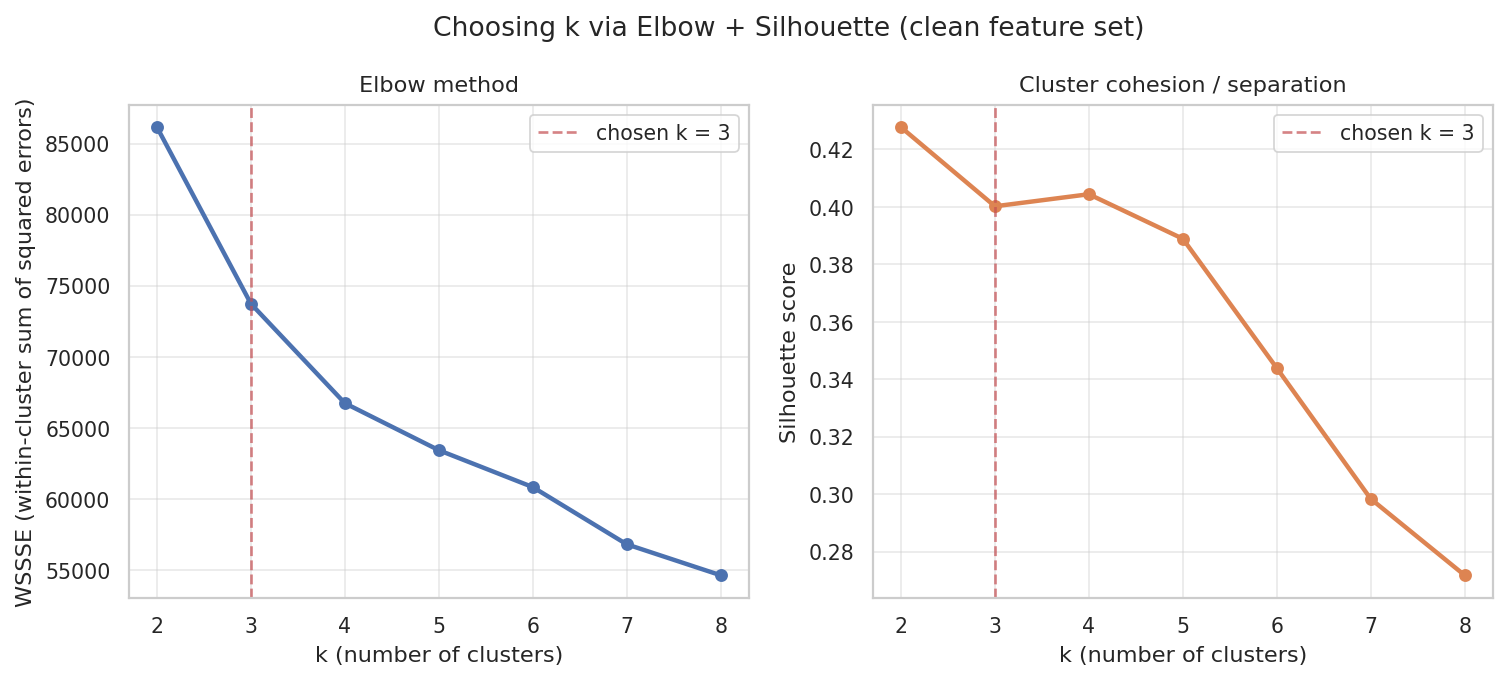
\includegraphics[width=0.95\linewidth]{01_elbow_silhouette.png}
  \caption{WSSSE (left) and silhouette (right) for $k \in \{2,\ldots,8\}$.
  WSSSE drops smoothly through the sweep but the silhouette peaks at
  $k=2$ ($0.43$) and stays high at $k=3$ ($0.40$) before degrading sharply
  beyond $k=5$. We select $k=3$.}
  \label{fig:elbow}
\end{figure}

We adopt $k=3$, which sacrifices only $0.03$ silhouette versus $k=2$ but
yields a meaningfully richer typology (a middle ``Experimenter'' tier
between Skeptic and Power User).

\subsection{Cluster geometry}

The three centroids are visually distinct in the 9-dimensional z-score
space:

\begin{figure}[H]
  \centering
  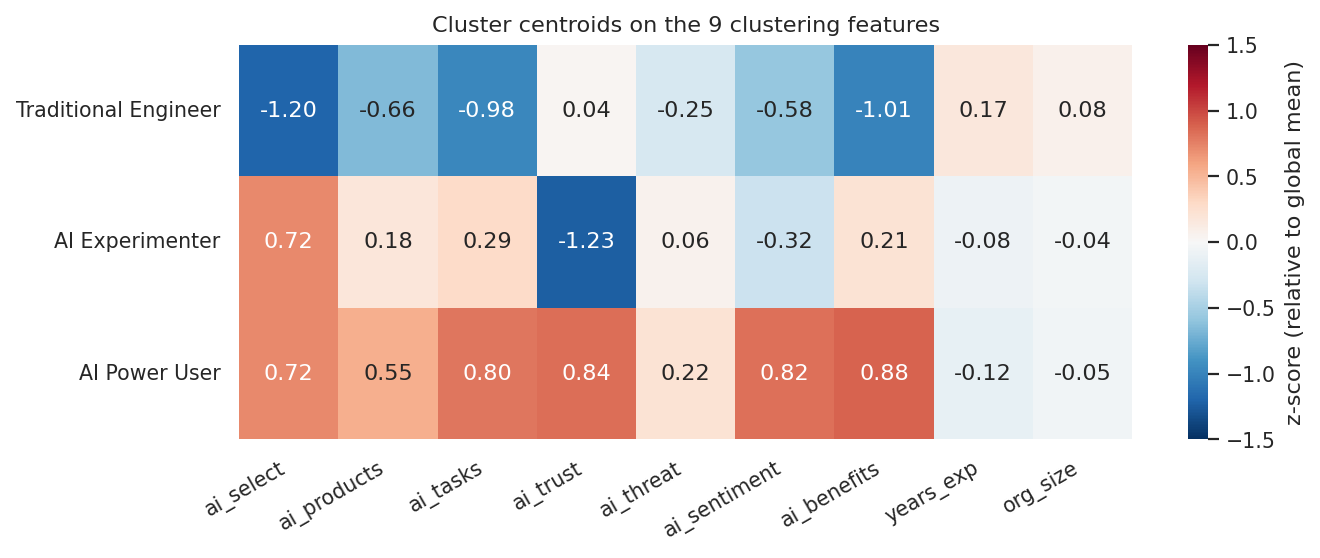
\includegraphics[width=0.95\linewidth]{02_centroid_heatmap.png}
  \caption{Cluster centroids on the nine clustering features (z-scores
  relative to the global mean). The Traditional Engineer is uniformly
  negative on every AI feature; the AI Power User is uniformly positive
  (notably trust = $+0.84$, benefit count = $+0.88$); the AI Experimenter
  occupies the middle on adoption but is \emph{distrustful} of AI accuracy
  ($z = -1.23$). The non-AI features (\texttt{years\_exp}, \texttt{org\_size})
  are nearly identical across clusters, confirming that clustering is
  driven by the AI dimensions, not by demographic confounds.}
  \label{fig:centroids}
\end{figure}

Cluster sizes are well-balanced
(Figure~\ref{fig:sizes}): no cluster is degenerate.

\begin{figure}[H]
  \centering
  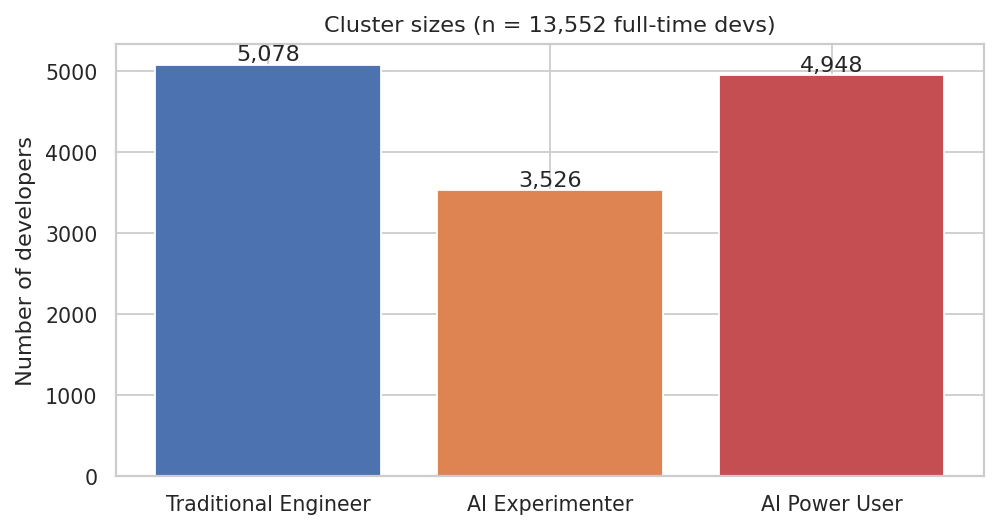
\includegraphics[width=0.75\linewidth]{03_cluster_sizes.png}
  \caption{Cluster sizes in the cleaned sample of 13{,}552 full-time
  developers (38\% / 26\% / 36\%).}
  \label{fig:sizes}
\end{figure}

\subsection{Headline outcomes per archetype}

\begin{figure}[H]
  \centering
  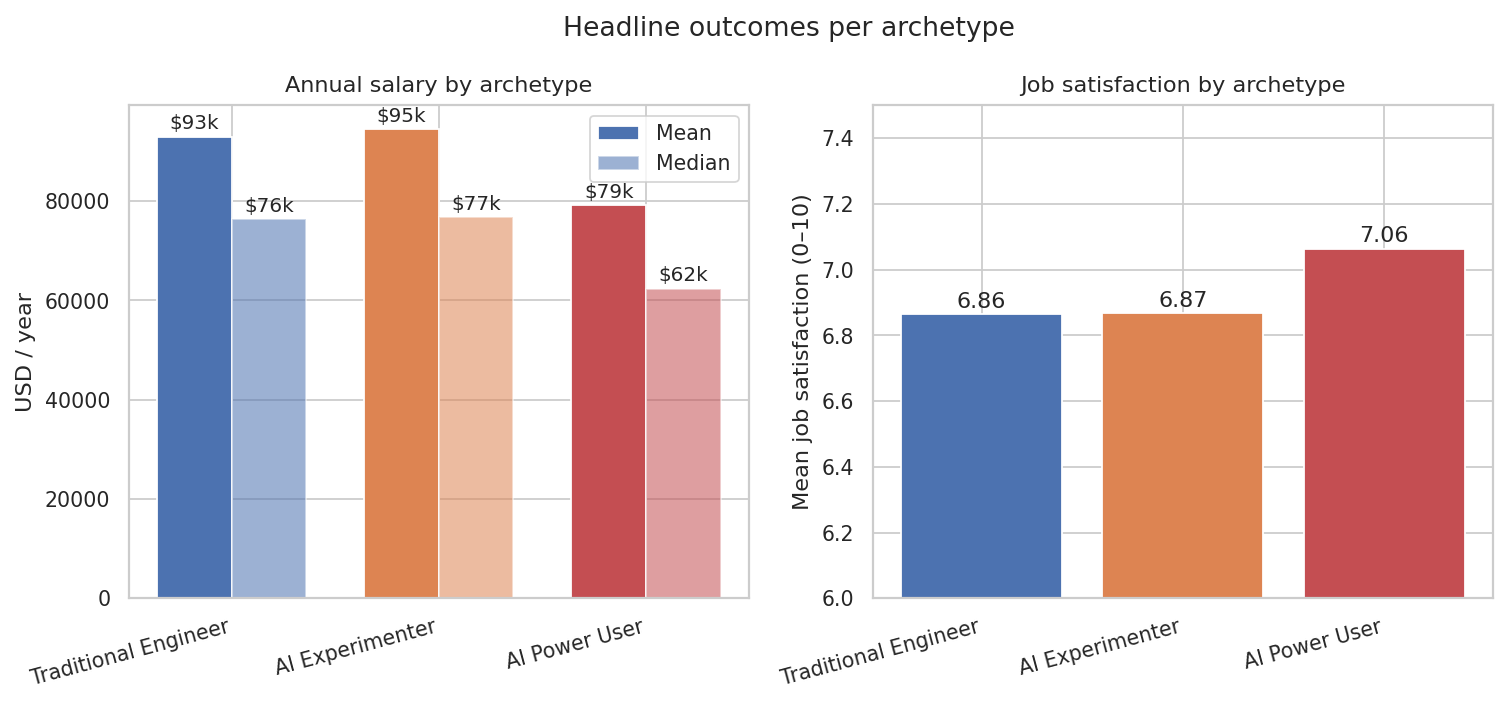
\includegraphics[width=0.95\linewidth]{04_salary_jobsat_per_archetype.png}
  \caption{Mean and median annual compensation (left) and job satisfaction
  on the 0--10 scale (right) per archetype.}
  \label{fig:salary-js}
\end{figure}

\begin{table}[H]
\centering
\caption{Headline outcomes per archetype.}
\rowcolors{2}{rowblue}{white}
\begin{tabular}{lrrrr}
\toprule
\textbf{Archetype} & \textbf{$n$} & \textbf{Mean salary} & \textbf{Median salary} & \textbf{JobSat (0--10)} \\
\midrule
Traditional Engineer & 5{,}078 & \$93{,}038 & \$76{,}433 & 6.86 \\
AI Experimenter      & 3{,}526 & \$94{,}570 & \$76{,}791 & 6.87 \\
AI Power User        & 4{,}948 & \$79{,}173 & \$62{,}402 & 7.06 \\
\bottomrule
\end{tabular}
\end{table}

\textbf{Surface read.} Power Users earn $\approx 15\%$ less than
Traditional Engineers, but report modestly higher job satisfaction
($+0.20$ on the 0--10 scale). The salary gap looks dramatic --- but the
deep-dive in Section~\ref{sec:deepdive} explains why it is largely an
experience confound.

\begin{figure}[H]
  \centering
  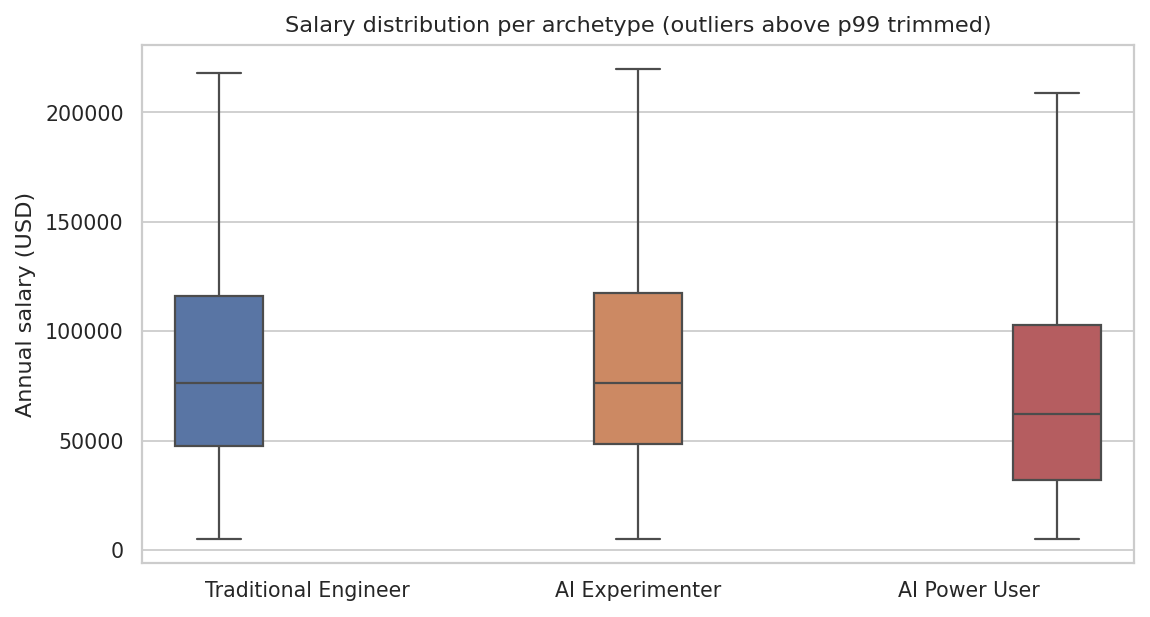
\includegraphics[width=0.85\linewidth]{11_salary_distribution_box.png}
  \caption{Boxplot of the salary distribution per archetype (outliers
  above the 99th percentile trimmed for legibility). Medians and IQRs
  overlap heavily; the difference between archetypes lies in the right
  tail.}
  \label{fig:box}
\end{figure}

\subsection{Deep dive --- does ``Power Users earn less'' survive controls?}
\label{sec:deepdive}

\subsubsection{Raw gradient by AI usage bin}

\begin{figure}[H]
  \centering
  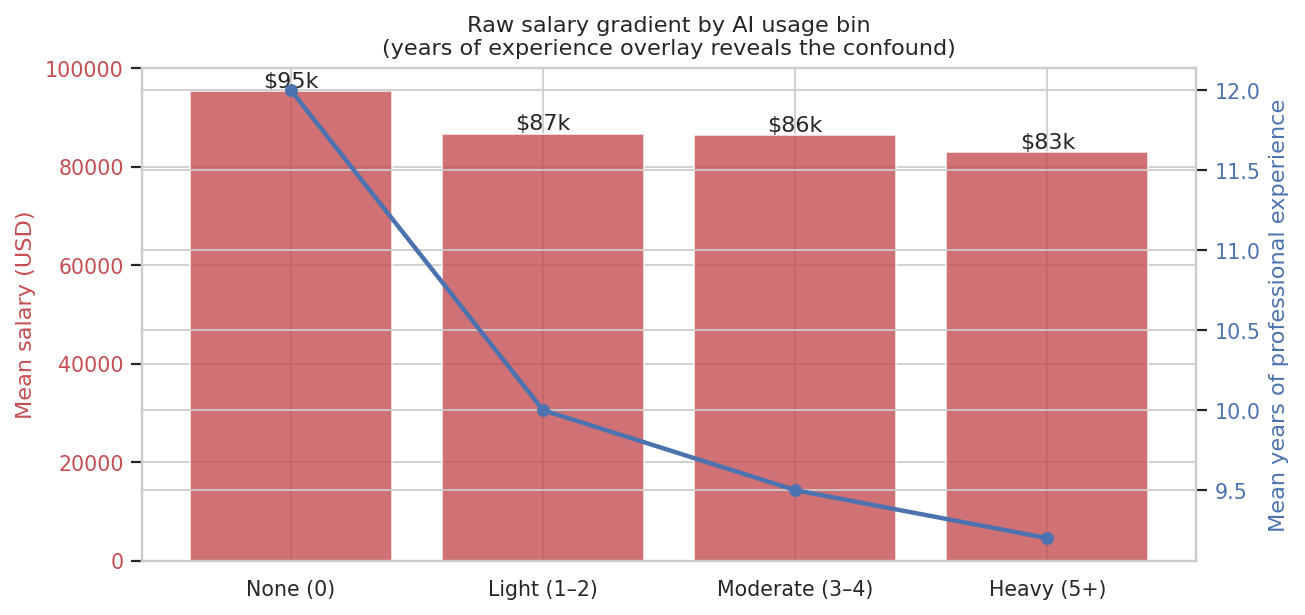
\includegraphics[width=0.85\linewidth]{05_salary_by_ai_usage.png}
  \caption{Bins by \emph{AI products used} (None / Light 1--2 /
  Moderate 3--4 / Heavy 5+). The salary curve drops monotonically
  ($\$95$k $\to$ $\$83$k); the overlaid years-of-experience line drops
  in lock-step ($12.0 \to 9.2$). This is the first warning that
  experience may be doing the work.}
  \label{fig:salary-by-ai}
\end{figure}

\subsubsection{Simpson's paradox by experience tier}

\begin{figure}[H]
  \centering
  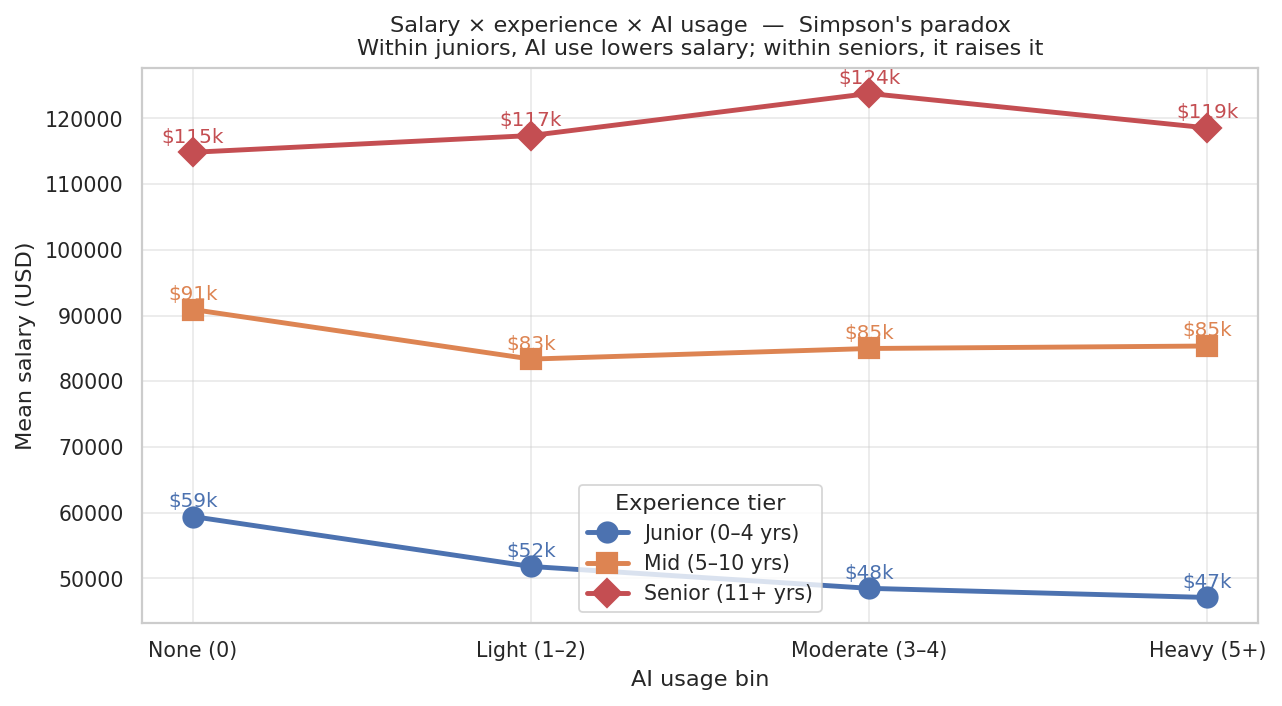
\includegraphics[width=0.95\linewidth]{06_simpsons_paradox.png}
  \caption{The headline figure of the project. Within each experience
  tier the salary--AI-usage relationship behaves differently: among
  juniors AI use lowers salary; among seniors it raises it.}
  \label{fig:simpsons}
\end{figure}

\begin{table}[H]
\centering
\caption{Mean salary (USD) by experience tier $\times$ AI usage bin.}
\rowcolors{2}{rowblue}{white}
\begin{tabular}{lrrrrl}
\toprule
\textbf{Experience} & \textbf{None} & \textbf{Light} & \textbf{Moderate} & \textbf{Heavy} & \textbf{Pattern} \\
\midrule
Junior (0--4 yrs) & \$59k & \$52k & \$48k & \$47k & Monotonic decline ($-\$12$k) \\
Mid (5--10 yrs)   & \$91k & \$83k & \$85k & \$85k & Light dip then flat \\
Senior (11+ yrs)  & \$115k & \$117k & \$124k & \$119k & Increase by $+\$4$k--$\$9$k \\
\bottomrule
\end{tabular}
\end{table}

Among juniors the popular ``AI Power Users earn less'' claim is real and
substantial. Among seniors it \textbf{reverses} --- the heaviest AI users
out-earn the abstainers by almost \$10k. The cell counts (601 to 2{,}583
per cell) are healthy, ruling out a small-sample artefact.

\subsubsection{Geography effect}

\begin{figure}[H]
  \centering
  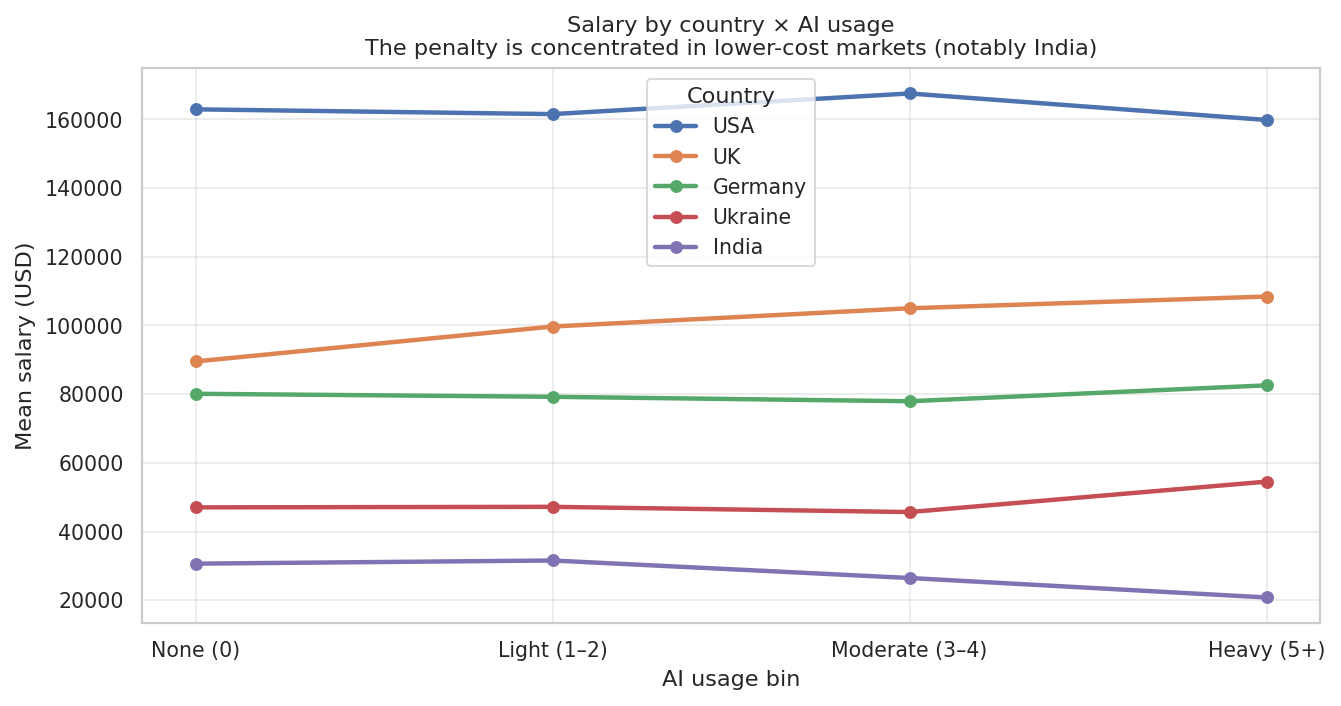
\includegraphics[width=0.95\linewidth]{07_country_x_ai.png}
  \caption{Salary across the top-5 countries, broken down by AI usage.
  The penalty is concentrated in lower-cost markets (notably India,
  $\$31$k $\to$ $\$21$k); in the highest-cost markets the relationship
  is flat (USA, Germany) or positive (UK, Ukraine).}
  \label{fig:country}
\end{figure}

The aggregate decline observed in the headline numbers is therefore
concentrated in the lowest-cost market in the top-5. In the highest-cost
markets the relationship is flat or positive.

\subsubsection{Role-mix effect}

\begin{figure}[H]
  \centering
  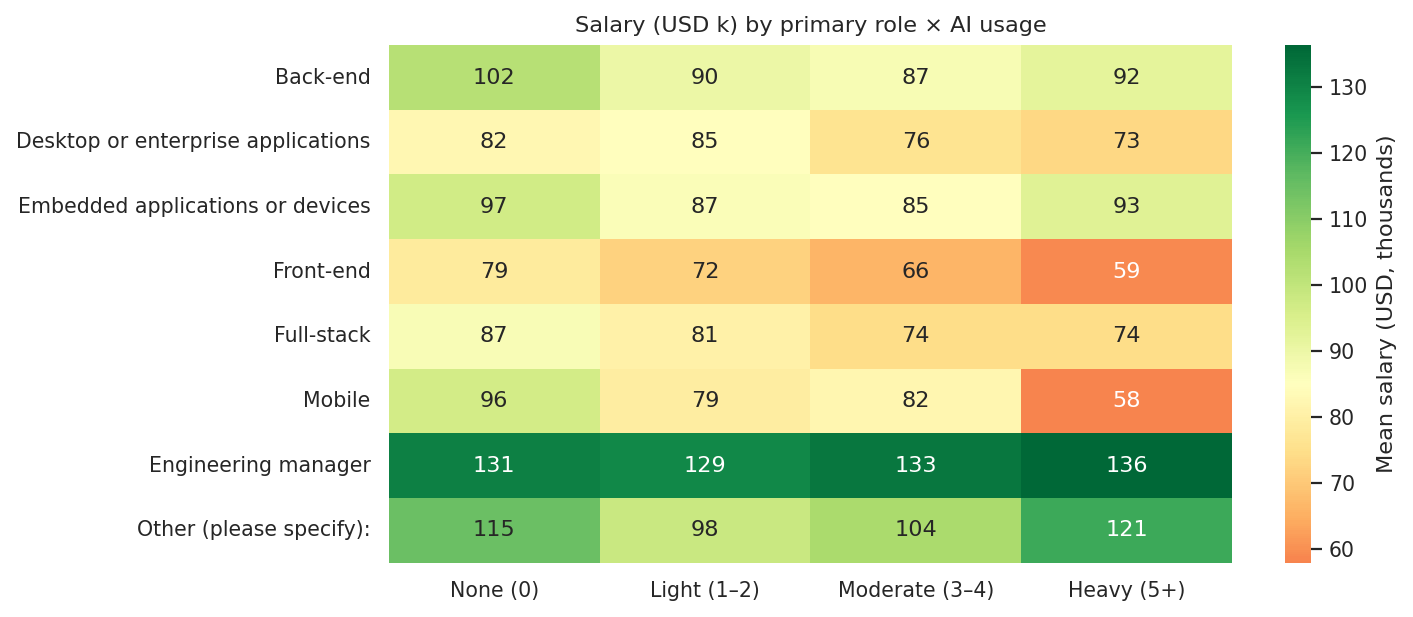
\includegraphics[width=0.95\linewidth]{08_role_x_ai_heatmap.png}
  \caption{Heatmap of mean salary (USD\,k) by primary developer role
  $\times$ AI usage bin. Most product roles (front-end, full-stack,
  mobile) decline with AI use; engineering managers show a small
  \emph{increase}; embedded developers are essentially flat.}
  \label{fig:role-heat}
\end{figure}

\subsubsection{Pearson correlations}

\begin{figure}[H]
  \centering
  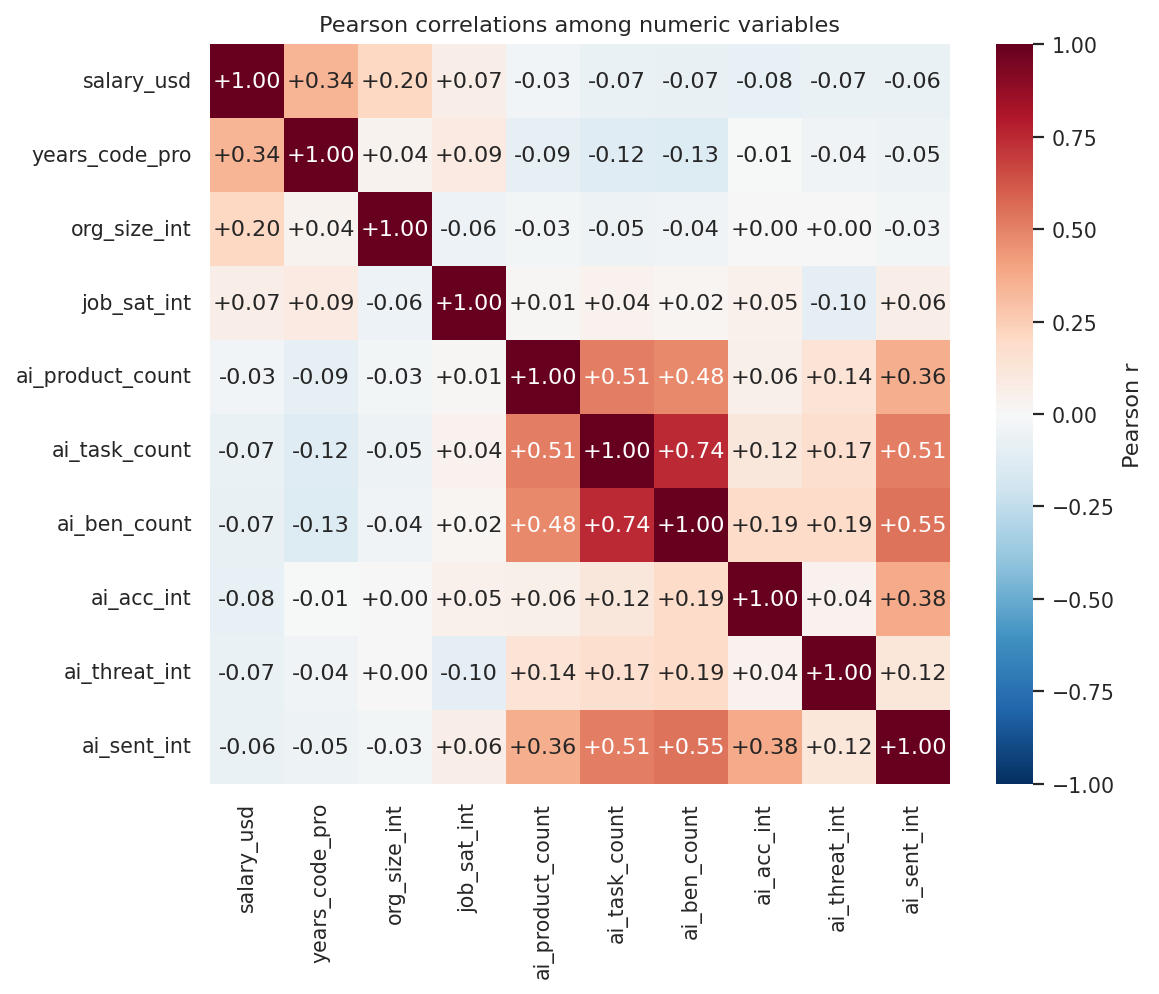
\includegraphics[width=0.85\linewidth]{09_correlation_matrix.png}
  \caption{Pearson correlations among the numeric variables. The strongest
  predictor of salary is \texttt{years\_code\_pro} ($r=+0.34$); every
  AI-positivity variable shows a small \emph{negative} correlation with
  salary ($-0.03$ to $-0.08$); the AI variables are highly inter-correlated
  (\texttt{ai\_task\_count} $\times$ \texttt{ai\_ben\_count} $= +0.74$).
  This justifies controlling for experience and org size in the regression.}
  \label{fig:corr}
\end{figure}

\subsubsection{Linear regression}
\label{sec:regression}

We fit a Spark MLlib \texttt{LinearRegression} of \emph{salary} on
\texttt{ai\_product\_count}, \texttt{ai\_task\_count},
\texttt{years\_code\_pro}, \texttt{org\_size\_int} (z-standardised inputs,
fit with \texttt{regParam = 0}):

\begin{equation}
\widehat{\text{salary}} = \beta_0
  + \beta_1 \cdot n_{\text{products}}
  + \beta_2 \cdot n_{\text{tasks}}
  + \beta_3 \cdot \text{years\_exp}
  + \beta_4 \cdot \text{org\_size}
\end{equation}

\begin{table}[H]
\centering
\caption{Linear regression coefficients. $R^2 = 0.155$; RMSE $=\$67{,}636$;
$N = 13{,}552$. ``\textbf{*}'' = $p<0.05$, ``\textbf{**}'' = $p<0.01$,
``\textbf{***}'' = $p<0.001$.}
\rowcolors{2}{rowblue}{white}
\begin{tabular}{lrrrrl}
\toprule
\textbf{Feature} & \textbf{Coef. (USD)} & \textbf{Std err} & \textbf{$t$} & \textbf{$p$} & \textbf{Sig.} \\
\midrule
\texttt{ai\_product\_count} & $+853$   & $432.2$ & $+1.97$  & $0.048$  & * \\
\texttt{ai\_task\_count}    & $-921$   & $290.5$ & $-3.17$  & $0.0015$ & ** \\
\texttt{years\_code\_pro}   & $+3{,}003$ & $71.8$  & $+41.85$ & $<0.0001$ & *** \\
\texttt{org\_size\_int}     & $+6{,}702$ & $277.7$ & $+24.13$ & $<0.0001$ & *** \\
\bottomrule
\end{tabular}
\end{table}

\begin{figure}[H]
  \centering
  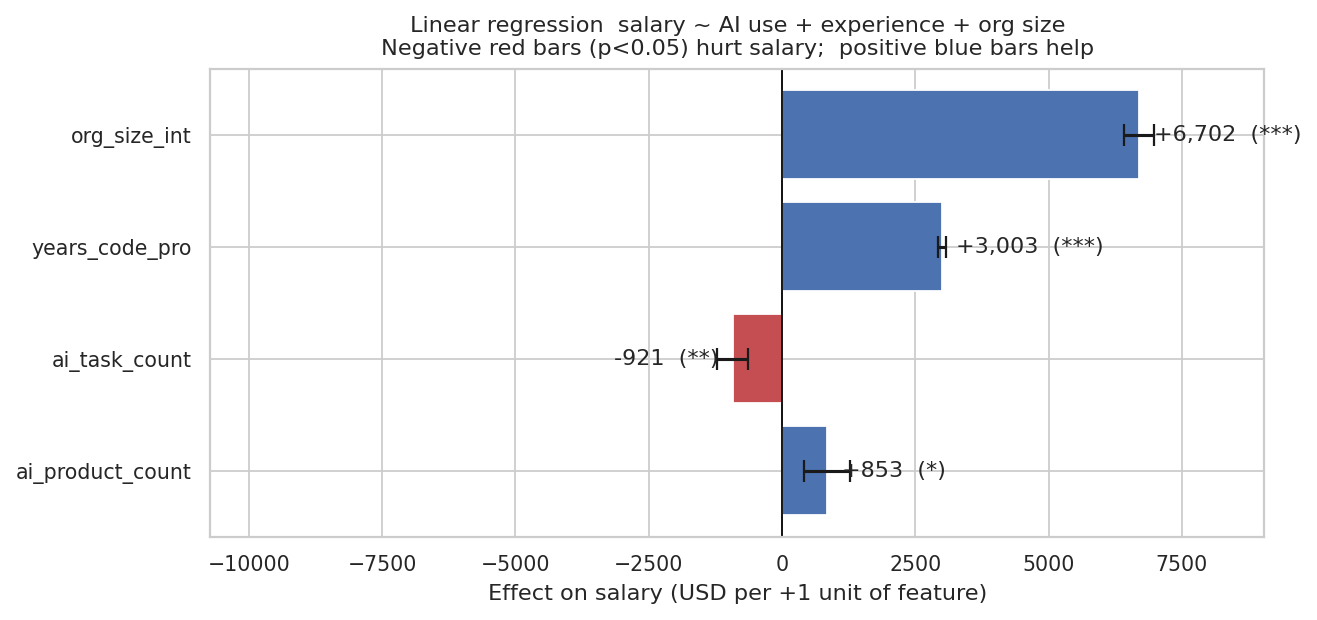
\includegraphics[width=0.95\linewidth]{10_regression_coefficients.png}
  \caption{Regression coefficients with $\pm 1$ std-error bars.
  Negative red bars (significant at $p<0.05$) hurt salary; positive blue
  bars help. After controlling for experience and org size, the number of
  AI products tried has a \emph{positive} effect on salary, while the
  number of work tasks delegated to AI has a \emph{negative} effect.}
  \label{fig:regression}
\end{figure}

\subsection{Demographic and contextual breakdowns}

\subsubsection{Primary developer role per archetype}

\begin{figure}[H]
  \centering
  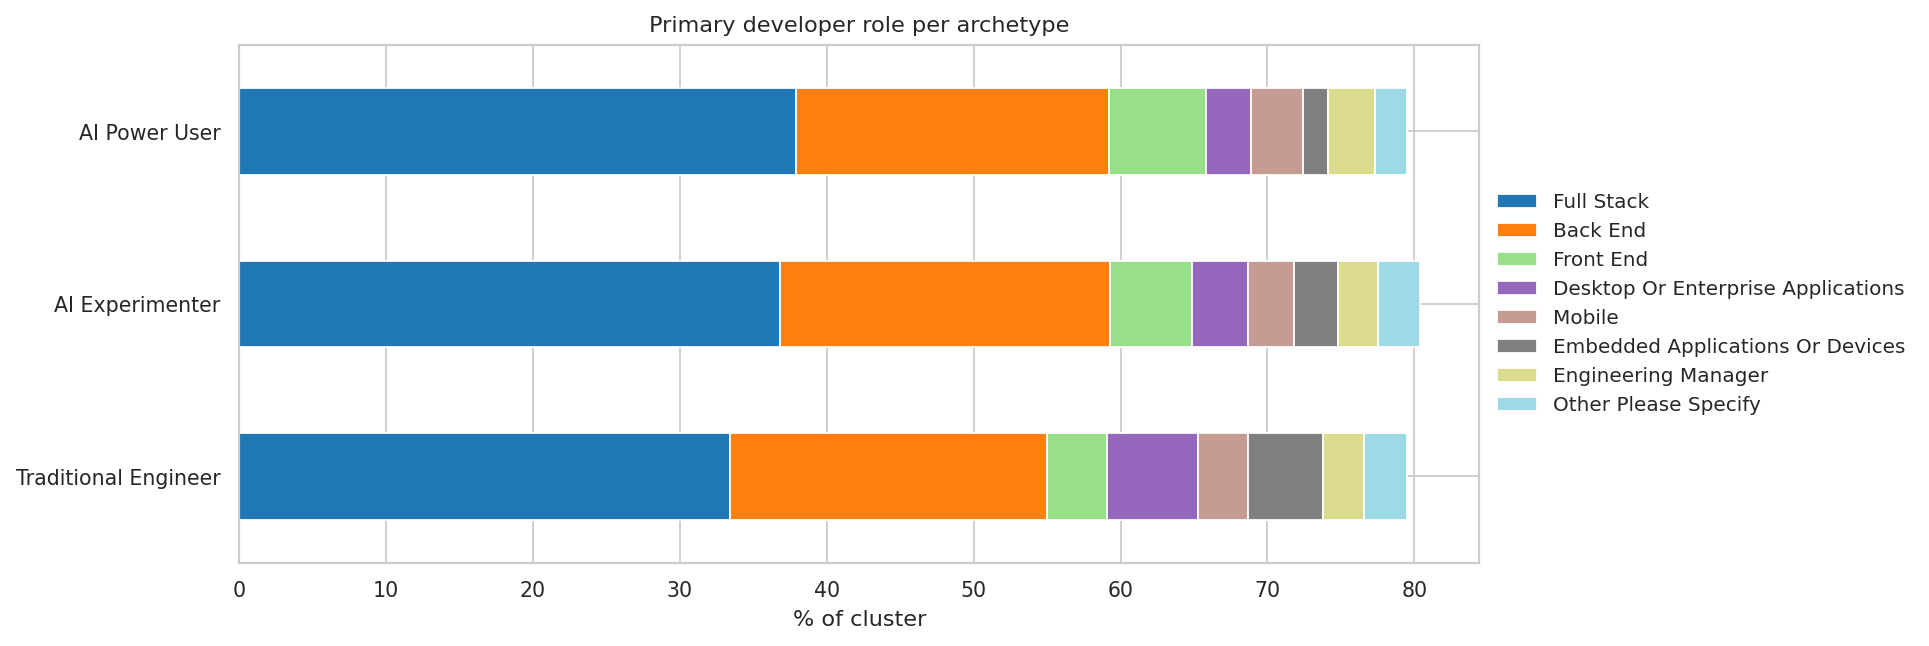
\includegraphics[width=\linewidth]{12_role_mix_per_archetype.png}
  \caption{Distribution of primary developer roles per cluster. AI Power
  User skews to full-stack (37.9\%) and front-end (6.6\%). Traditional
  Engineer over-indexes on desktop / enterprise (6.2\% vs 3.1\%) and
  embedded (5.1\% vs 1.7\%) --- embedded developers are $3\times$ more
  likely to be Traditional Engineers than AI Power Users.}
  \label{fig:role-mix}
\end{figure}

\subsubsection{Remote-work mix per archetype}

\begin{figure}[H]
  \centering
  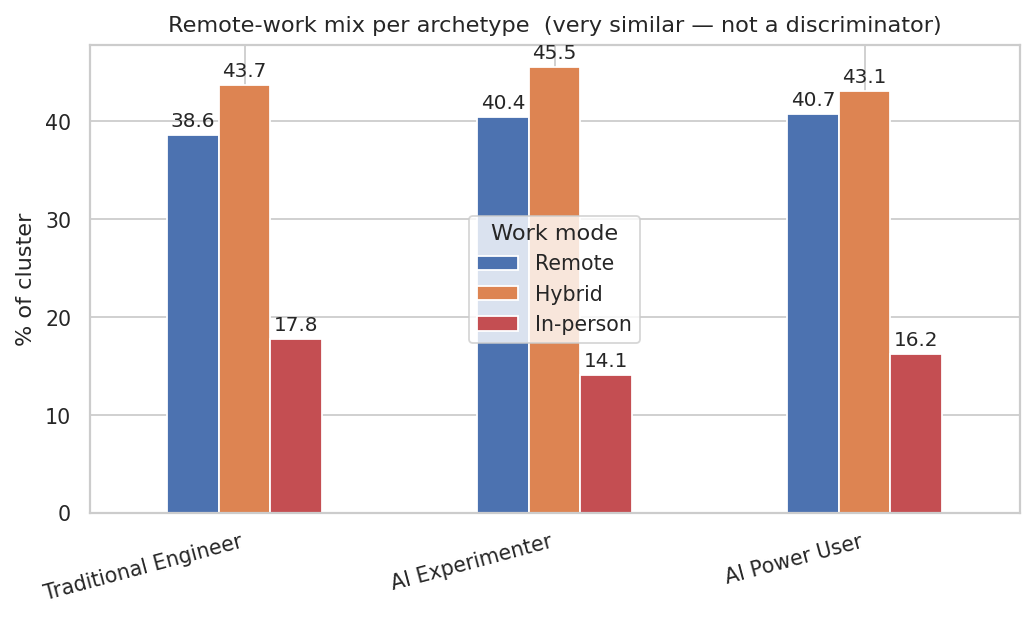
\includegraphics[width=0.85\linewidth]{13_remote_work_per_archetype.png}
  \caption{Remote / Hybrid / In-person mix per archetype is almost
  identical across clusters (within 2--3 percentage points). AI archetype
  membership does \emph{not} predict work mode.}
  \label{fig:remote}
\end{figure}

\subsubsection{Self-identification (\texttt{MainBranch})}

After filtering to full-time employed developers, hobbyists and learners
are correctly excluded; the remaining variation is between \emph{primary
developer} (93--96\%) and \emph{occasional coder} (4--7\%). Traditional
Engineers contain the largest share of occasional coders (7.0\%),
consistent with their lower AI engagement and broader role mix
(DBAs, sysadmins, embedded specialists).

% ════════════════════════════════════════════════════════════════════════════
\section{Discussion}
% ════════════════════════════════════════════════════════════════════════════

\subsection{The reframed thesis}

The original ``Hype vs Maturity'' project goal --- measuring how hyped vs
mature \emph{companies} affect their employees --- turned out to be
impossible on this dataset because the unit of observation is the
\emph{individual}. The adapted thesis (developer archetypes,
individual-level AI adoption) proved tractable and produced three crisply
separated clusters (silhouette $= 0.40$).

The most interesting finding is \textbf{not} the headline number (Power
Users earn 15\% less). That number is real but partly an artefact of
where AI adoption has spread: into junior developers and lower-cost
markets. The finding that survives every control we apply is more nuanced
and arguably more useful:

\begin{quote}\itshape
  Trying more AI products is associated with slightly higher
  compensation, but offloading more of one's work to AI is associated
  with slightly lower compensation, after controlling for experience
  and org size.
\end{quote}

In Spark-ML units, the marginal effect on annual salary of a single
extra task offloaded to AI is $-\$921$ ($p=0.0015$); the marginal effect
of trying one additional product is $+\$853$ ($p=0.048$). The contrast
between these two coefficients is the analytical kernel of the report.

\subsection{Limitations}

\begin{enumerate}[leftmargin=2em]
  \item \textbf{Causal direction is unidentified.} Workers earning less
        might compensate by leaning harder on AI, rather than AI use
        causing lower pay. The regression is observational, not an
        instrument.
  \item \textbf{\texttt{ConvertedCompYearly} is volatile.} It is
        normalised to USD by Stack Overflow's currency table, but
        cost-of-living, equity, and benefits are excluded. The Indian
        market collapse in Figure~\ref{fig:country} may be over-stated
        for this reason.
  \item \textbf{Multi-valued columns are reduced to first-of-list.}
        Dev role uses the first listed \texttt{DevType} as the ``primary
        role''; the survey does not enforce ordering, so this is
        approximate.
  \item \textbf{$k=3$ sacrifices 0.03 silhouette versus $k=2$.} It
        produces a richer typology, but two-cluster solutions are
        technically more compact.
  \item \textbf{Job satisfaction is on a 0--10 scale and shows almost no
        variance across clusters.} Any ``satisfaction'' claims rest on a
        narrow $\approx 0.2$-point band.
\end{enumerate}

\subsection{Implications}

\begin{itemize}[leftmargin=2em]
  \item For developers: \emph{trying} the latest assistants is at worst
        neutral and likely modestly positive for compensation, but
        \emph{structural delegation} of one's job to those tools is a
        separate behaviour that empirically tracks with lower pay.
  \item For employers and tooling vendors: the largest population that
        has adopted AI tooling is junior front-end and full-stack
        developers in emerging markets. Productivity claims targeted at
        this segment cannot be assumed to transfer to senior or
        hardware-adjacent engineers.
  \item For the AI hype-vs-maturity discourse: the data does not support
        a binary opposition. The structure is graded along an adoption
        axis with two distinct sub-behaviours (tool curiosity vs task
        delegation) that move salary in opposite directions.
\end{itemize}

% ════════════════════════════════════════════════════════════════════════════
\section{Conclusion}
% ════════════════════════════════════════════════════════════════════════════

We applied an end-to-end Spark/Scala big-data pipeline --- CSV ingestion,
DataFrame cleaning, MLlib feature scaling, K-Means clustering, RDD
aggregations, and \texttt{LinearRegression} modelling --- to the 2024
Stack Overflow Developer Survey, recovering three latent developer
archetypes (Traditional Engineer, AI Experimenter, AI Power User) with a
silhouette score of $0.40$ and balanced cluster sizes.

The popular claim that \emph{AI Power Users earn less} is technically
true at the population level ($-\$15$k versus Traditional Engineers) but
is shown to be a Simpson's paradox: among juniors the gap is real
($-\$12$k from None to Heavy), among seniors it reverses ($+\$9$k). A
controlled regression decomposes the AI signal into two components with
opposite salary effects: trying more products ($+\$853$, $p=0.05$) helps,
while delegating more tasks to AI ($-\$921$, $p=0.0015$) hurts.
Remote-work mode does not vary with archetype.

All artefacts --- Spark code, summary CSVs, the labelled per-respondent
Parquet, plot scripts, and 13 publication-quality figures --- are
reproducible from a single \texttt{sbt run} followed by
\texttt{python3 scripts/make\_plots.py}.

% ════════════════════════════════════════════════════════════════════════════
\appendix
\section{Reproducing the analysis}
% ════════════════════════════════════════════════════════════════════════════

\begin{lstlisting}[language=bash, caption={Build, run, plot.}]
# 1. Place the survey CSV
cp survey_results_public.csv data/dataset.csv

# 2. Build & run the pipeline (Java 11 required)
JAVA_HOME=/usr/lib/jvm/jdk-11.0.30-oracle-x64 sbt "runMain ecosystem.Main"

# 3. Generate the figures
python3 -m venv .venv-plot && source .venv-plot/bin/activate
pip install pandas matplotlib pyarrow seaborn
python3 scripts/make_plots.py
\end{lstlisting}

Outputs land under \texttt{output/report/} (CSV $+$ Parquet) and
\texttt{output/figures/} (PNG).

\section{Repository layout}

\begin{lstlisting}[language=bash]
build.sbt
data/dataset.csv                 # Stack Overflow 2024 raw CSV (gitignored)
output/
  report/                        # 17 summary CSV directories + Parquet
  figures/                       # 13 PNG plots
  run.log                        # captured stdout of the pipeline
report/main.tex                  # this file
scripts/make_plots.py            # matplotlib / seaborn figure generator
src/main/scala/ecosystem/
  Main.scala                     # pipeline entry point
  Cleaning.scala                 # schema-aware filtering + ordinal encoding
  Features.scala                 # VectorAssembler + StandardScaler
  OptimalK.scala                 # elbow + silhouette sweep
  Clustering.scala               # final K-Means + archetype labels
  Analysis.scala                 # multi-section impact report (DF + RDD + LR)
\end{lstlisting}

% ════════════════════════════════════════════════════════════════════════════
\section*{References}
% ════════════════════════════════════════════════════════════════════════════
\addcontentsline{toc}{section}{References}

\begin{thebibliography}{9}

\bibitem{stackoverflow2024}
Stack Overflow,
\textit{Stack Overflow Developer Survey 2024},
\url{https://survey.stackoverflow.co/2024}, accessed May 2026.

\bibitem{spark}
M.~Zaharia et~al.,
``Apache Spark: A Unified Engine for Big Data Processing,''
\textit{Communications of the ACM}, vol.~59, no.~11, pp.~56--65, 2016.

\bibitem{mllib}
X.~Meng et~al.,
``MLlib: Machine Learning in Apache Spark,''
\textit{Journal of Machine Learning Research}, vol.~17, no.~34, pp.~1--7, 2016.

\bibitem{kmeans}
J.~MacQueen,
``Some Methods for Classification and Analysis of Multivariate Observations,''
\textit{Proceedings of the 5th Berkeley Symposium on Mathematical Statistics
and Probability}, vol.~1, pp.~281--297, 1967.

\bibitem{silhouette}
P.~J.~Rousseeuw,
``Silhouettes: A Graphical Aid to the Interpretation and Validation of
Cluster Analysis,''
\textit{Journal of Computational and Applied Mathematics},
vol.~20, pp.~53--65, 1987.

\bibitem{simpson}
E.~H.~Simpson,
``The Interpretation of Interaction in Contingency Tables,''
\textit{Journal of the Royal Statistical Society, Series B},
vol.~13, no.~2, pp.~238--241, 1951.

\bibitem{eslii}
T.~Hastie, R.~Tibshirani, and J.~Friedman,
\textit{The Elements of Statistical Learning}, 2nd ed.,
Springer, 2009.

\end{thebibliography}

\end{document}
